\chapter{\label{app2:theory}Appendix}


urrent research in joint action suggest that interoceptive predictive processes are at the core of successful human social interactions \citep{Graziano2013,Manera2013,Sparenberg2012,Springer2012}.  The essence of this proposal is that we use our own cognitive resources to build mental models of other people’s cognitions and the shared tasks that we share with others \citep{Tomasello2005a}.  Simulation of other people’s cognitive states (e.g., what they are feeling, thinking, and attending, a.k.a. a theory of mind) guide our expectations about their future behaviour, and in this way contribute to the viability of social interactions.



\section{Predictive coding\label{app2:predictiveCoding}}

PC first emerged as a data processing and compression strategy in computer science \citep{Rao1999}.  Researchers programmed a multi-layer artificial neural network to use downwards connections to match samples of .JPEG images with successful predictions. Visual signals were processed via a hierarchical system in which each level tried to predict activity at the level below it using recurrent feedback connections. If the feedback successfully predicted the lower-level activity, no further action was required. Failure of the model to predict the visual signal resulted in tuning and revision of the model using ``residual errors'' derived from the discrepancy between top-down predictions and lower-level activity.  Predictive coding offered a much more computationally efficient mechanism for data processing, because prediction errors were the only informational novelties in the system \citep{Clark2015}.









\section{Motor control\label{app2:motorControl}}
Successful regulation with the environment depends on an organism's capacity to move from its current state to a desired state.  In the case of the human evolutionary niche, organismic regulation hinges largely on movement, be it physical or simulated \citep{Wolpert1995}.

Theories of motor control generally agree the brain generates ``forward models'' that anticipate perceptual inputs and desired motor states \citep{Pickering2014}. The first paradigmatic theory of motor control suggested that forward models for action relied on special-purpose mechanism auxiliary to core mechanisms of perception of action \citep{Wolpert1997}.  This hypothesis, now known as the Auxiliary Forward Models \citep[AFM, see][]{Pickering2014}, relies on a dual mechanism of motor control.  First, a motor command is estimated in the brain by an ``inverse model,'' which contains as its inputs both the desired state and the actual state of the organism (e.g., the position of the body, see Figure ~\ref{fig:AFM}).  When the motor command is generated, an auxiliary copy (i.e., an ``efference copy'') is also generated, and is sent to a forward model which then generates predictions about action and perception by simulating the musculoskeletal system and contextual environment \citep{Wolpert1995,Blakemore1998,Flanagan2003}.  Prediction error arising from a discrepancy between predicted and resultant sensory inputs are then used as feedback to inform the generation of the next motor command in the inverse model, and so on in a loop, until the fit between sensory prediction and input is sharpened.

A more recent alternative proposal to the AFM suggests that forward models, instead of being auxiliary to, may instead lie at the heart of all forms of perception and action \citep{Friston2010}.  In contrast to AFM, the ``Integrative Forward Models'' account of motor control \citep[IFM, see][]{Pickering2014} posits that predictions from forward models act directly as action commands.  There is no dedicated mechanism used to predict the outcomes of our own (or others’) actions in addition to the action commands themselves.  Instead, generative action-oriented models are treated as the actual state of affairs, and cause a cascade of downward predictions about what should be the state of the models in the levels below (see Figure ~\ref{fig:IFM}).  In the IFM approach, there is no need for a motor command or efference copy at each level of action prediction, and prediction errors directly update the action models themselves.



\begin{figure}[htbp]
  \begin{center}
    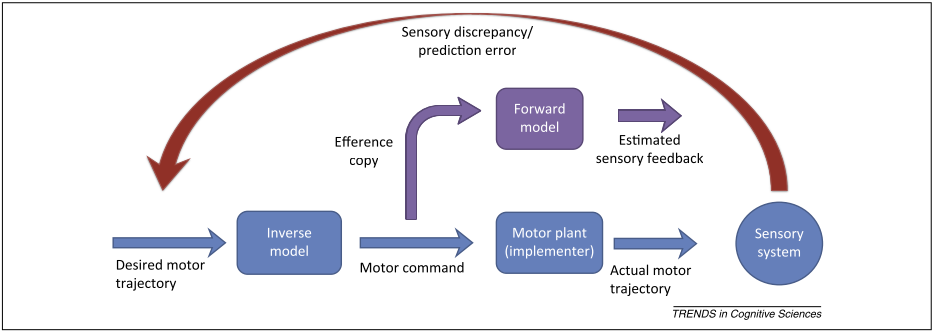
\includegraphics[scale=.5]{images/AFM.png}
      \caption{The Auxiliary Forward Model of motor control}
        \label{fig:AFM}
   \end{center}
\end{figure}

\begin{figure}[htbp]
  \begin{center}
    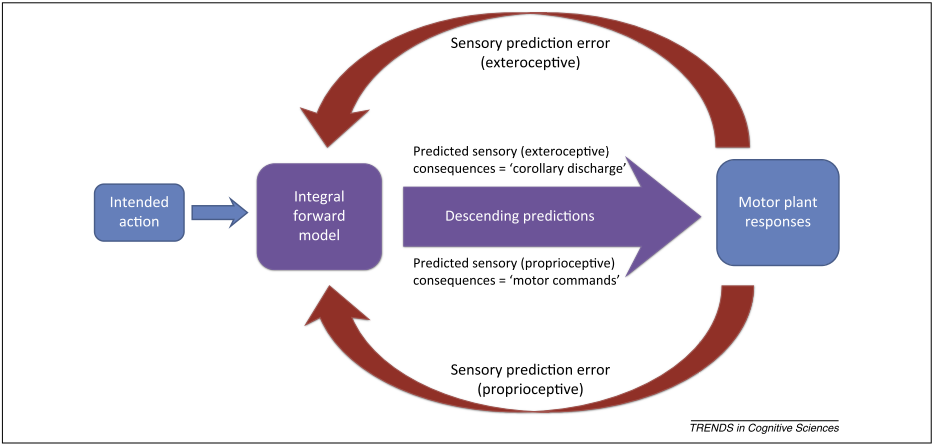
\includegraphics[scale=.5]{images/IFM.png}
      \caption{The Integrated Forward Model of motor control}
        \label{fig:IFM}
   \end{center}
\end{figure}


Both the AFM and IFM approaches agree that prediction, error minimisation, and hierarchical modelling are core processes in human cognition. From a thermodynamic standpoint, however, IFM appears to offer a more efficient model for free energy minimisation.  By replacing motor commands with direct predictions about proprioceptive and exteroceptive consequences, the need for a distinct optimal control calculation (i.e. an inverse model) disappears and along with it the need for an efference copy of the motor command, thus implicitly minimising various energetic costs \citep{Pickering2014,Friston2010}.   In place of the auxiliary mechanisms of the AFM, IFM posit a more complex (distributed) forward model mapping prior beliefs about desired trajectories to sensory consequences.  Whereas the ``heavy lifting'' in AFM required the use of an efference copy and inverse models, in IFM this work is done by the acquisition and use of a more complex predictive (generative) model \citep{Pickering2014}.

%According to the AFM account, the forward model is distinct from the inverse model, because it involves apparatus that computes the motor commands used to drive online action. Such a model is thus free to depart considerably in form from whatever governs the true kinematics of the agent.  Furthermore (in AFMs) the outputs of the forward model (i.e., the corollary discharge) do not cause movements – they are just used to finesse and predict outcomes and in learning.

%Comparisons between downward sweeps of prediction and upward sweeps of sensory input lead to a cascade of error signals throughout the hierarchy. These error signals are used to adjust the forward models that are guiding action execution (Clark, 2013). Importantly, actions are aimed at minimising prediction errors, by matching sensory inputs to predictions— a process termed active inference (Friston, 2008;Friston & Frith, 2015a, b). Eventually, active inference leads iteratively to a solution that will take the organism from its current motor state to the desired one.
